\documentclass[twocolumn]{article}
\usepackage[utf8]{inputenc}
\usepackage[margin=0.5in]{geometry}

% href
\usepackage{hyperref}
\hypersetup{
    colorlinks=true,
    linkcolor=black,
    citecolor=black,
    filecolor=magenta,      
    urlcolor=cyan,
    pdfpagemode=FullScreen,
    }

% figures
\usepackage{graphicx}

\title{Day02 Exercise}
\date{March 2022}

\begin{document}

\maketitle

\section{Introduction} \label{sec:intro}

Your goal is to reverse-engineer this document! Here's what to do:

\begin{enumerate}
    \item Open Overleaf, sign in.
    \item Create a blank project by:
    \begin{enumerate}
        \item Clicking on ``New Project" 
        \item Clicking on ``Blank Project"
    \end{enumerate}
    \item Fill in the project so it looks like this page!
\end{enumerate}

\section{Use a \texttt{figure} environment} \label{sec:figure}

Replicate Figure~\ref{fig:universe}.

\begin{figure}[h]
    \centering
    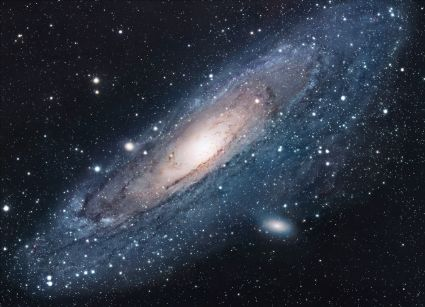
\includegraphics[width=0.8\linewidth]{images/universe.jpg}
    \caption{The universe is big!}
    \label{fig:universe}
\end{figure}

\section{Create a \texttt{table}} \label{sec:table}

Replicate Table~\ref{tab:mpg}.

\begin{table}[h]
    \centering
    \begin{tabular}{c|c|c|c}
        \textbf{Manufacturer} & \textbf{Model} & \textbf{City} & \textbf{Highway} \\ \hline
        Audi       & A4        & 18 & 27 \\ \hline
        Subaru     & Impreza   & 20 & 27 \\ \hline
        Toyota     & Corolla   & 26 & 35 \\ \hline
        Volkswagen & GTI       & 22 & 29 \\
    \end{tabular}
    \caption{Fuel mileage for 2008 compact vehicles.}
    \label{tab:mpg}
\end{table}

\section{Equations and Citations} \label{sec:eq_cite}

Write the following definition of entropy, $H$, from \cite{ref:shannon1948},

\begin{equation}
    H = -\sum_i p_i \log p_i
\end{equation}
where $p_i$ is the probability of the $i$-th outcome.

\bibliographystyle{ieeetr}
\bibliography{example}

\section*{Hints}

Unless you want more practice, you don't have to replicate this section!

\begin{itemize}
    \item \textbf{Formatting}
    \begin{itemize}
        \item The numbered headers use \texttt{section} commands.
        \item The margins have been adjusted to 0.5 in.
        \item The \texttt{[twocolumn]} option for \texttt{documentclass} creates two columns.
        \item Text formatting we've used includes \texttt{texttt}.
    \end{itemize}
    \item \textbf{\ref{sec:intro} Introduction}
    \begin{itemize}
        \item There is a nested \texttt{enumerate} environment here!
    \end{itemize}
    \item \textbf{\ref{sec:figure} Use a \texttt{figure} environment}
    \begin{itemize}
        \item To get the image of the universe, you can download the image \href{github.com/mdelrosa/latex101/blob/master/day02/exercise/images/universe.jpg}{from Github}.
        \item To center the figure, use the \texttt{\textbackslash centering} command.
        \item To control the width of the \texttt{float}, use the \texttt{[width=\textbackslash linewidth]} option with the \texttt{\textbackslash includegraphics} command.
    \end{itemize}
    \item \textbf{\ref{sec:table} Create a \texttt{table}}
    \begin{itemize}
        \item If it's helpful, then use \href{https://www.tablesgenerator.com/}{tablesgenerator.com}.
        \item Don't forget to make the headers bold!
    \end{itemize}
    \item \textbf{\ref{sec:eq_cite} Equations and Citations}
    \begin{itemize}
        \item If you need help finding symbols, then try \href{http://detexify.kirelabs.org/classify.html) }{detexify}.
        \item Download the database file (\texttt{example.bib}) \href{github.com/mdelrosa/latex101/blob/master/day02/exercise/example.bib}{from Github}.
        \item Don't forget to call \texttt{\textbackslash bibliographystyle\{ieeetr\}} and \texttt{\textbackslash bibliography\{example\}}
    \end{itemize}
\end{itemize}

\end{document}